\documentclass[ignorenonframetext,]{beamer}
\setbeamertemplate{caption}[numbered]
\setbeamertemplate{caption label separator}{: }
\setbeamercolor{caption name}{fg=normal text.fg}
\beamertemplatenavigationsymbolsempty
\usepackage{lmodern}
\usepackage{amssymb,amsmath}
\usepackage{ifxetex,ifluatex}
\usepackage{fixltx2e} % provides \textsubscript
\ifnum 0\ifxetex 1\fi\ifluatex 1\fi=0 % if pdftex
  \usepackage[T1]{fontenc}
  \usepackage[utf8]{inputenc}
\else % if luatex or xelatex
  \ifxetex
    \usepackage{mathspec}
  \else
    \usepackage{fontspec}
  \fi
  \defaultfontfeatures{Ligatures=TeX,Scale=MatchLowercase}
\fi
% use upquote if available, for straight quotes in verbatim environments
\IfFileExists{upquote.sty}{\usepackage{upquote}}{}
% use microtype if available
\IfFileExists{microtype.sty}{%
\usepackage{microtype}
\UseMicrotypeSet[protrusion]{basicmath} % disable protrusion for tt fonts
}{}
\newif\ifbibliography
\hypersetup{
            pdftitle={Procesos Estocásticos},
            pdfauthor={Kamal Romero},
            pdfborder={0 0 0},
            breaklinks=true}
\urlstyle{same}  % don't use monospace font for urls
\usepackage{graphicx,grffile}
\makeatletter
\def\maxwidth{\ifdim\Gin@nat@width>\linewidth\linewidth\else\Gin@nat@width\fi}
\def\maxheight{\ifdim\Gin@nat@height>\textheight0.8\textheight\else\Gin@nat@height\fi}
\makeatother
% Scale images if necessary, so that they will not overflow the page
% margins by default, and it is still possible to overwrite the defaults
% using explicit options in \includegraphics[width, height, ...]{}
\setkeys{Gin}{width=\maxwidth,height=\maxheight,keepaspectratio}

% Prevent slide breaks in the middle of a paragraph:
\widowpenalties 1 10000
\raggedbottom

\AtBeginPart{
  \let\insertpartnumber\relax
  \let\partname\relax
  \frame{\partpage}
}
\AtBeginSection{
  \ifbibliography
  \else
    \let\insertsectionnumber\relax
    \let\sectionname\relax
    \frame{\sectionpage}
  \fi
}
\AtBeginSubsection{
  \let\insertsubsectionnumber\relax
  \let\subsectionname\relax
  \frame{\subsectionpage}
}

\setlength{\parindent}{0pt}
\setlength{\parskip}{6pt plus 2pt minus 1pt}
\setlength{\emergencystretch}{3em}  % prevent overfull lines
\providecommand{\tightlist}{%
  \setlength{\itemsep}{0pt}\setlength{\parskip}{0pt}}
\setcounter{secnumdepth}{0}

\title{Procesos Estocásticos}
\subtitle{Econometría II}
\author{Kamal Romero}
\date{(actualizado: 2021-09-09)}

\begin{document}
\frame{\titlepage}

\begin{frame}{Tipo de Cambio Nominal}

\begin{itemize}
\tightlist
\item
  El comportamiento del tipo de cambio es lejos de ser sistemático y
  predecible
\end{itemize}

\begin{center}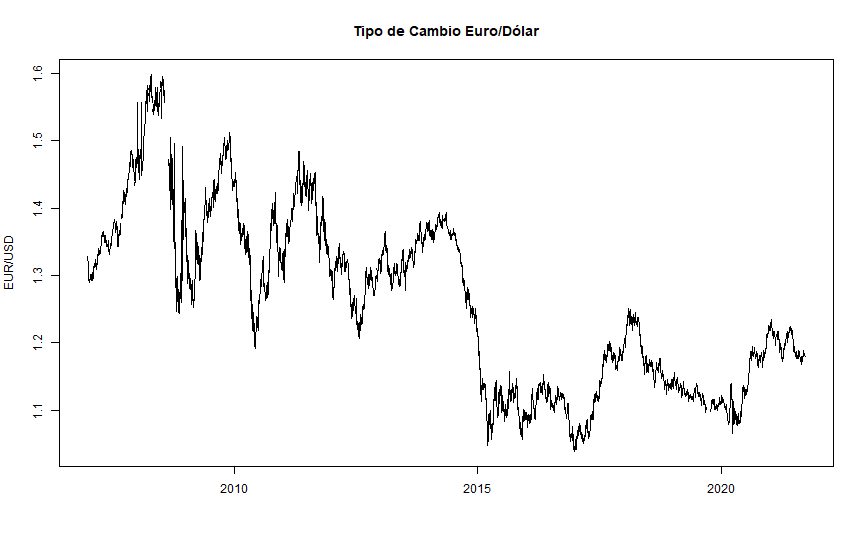
\includegraphics{Procesos_estocasticos_files/figure-beamer/er1-1} \end{center}

\end{frame}

\begin{frame}{Tipo de Cambio Nominal}

\begin{itemize}
\tightlist
\item
  El comportamiento del tipo de cambio es lejos de ser sistemático y
  predecible
\end{itemize}

\begin{center}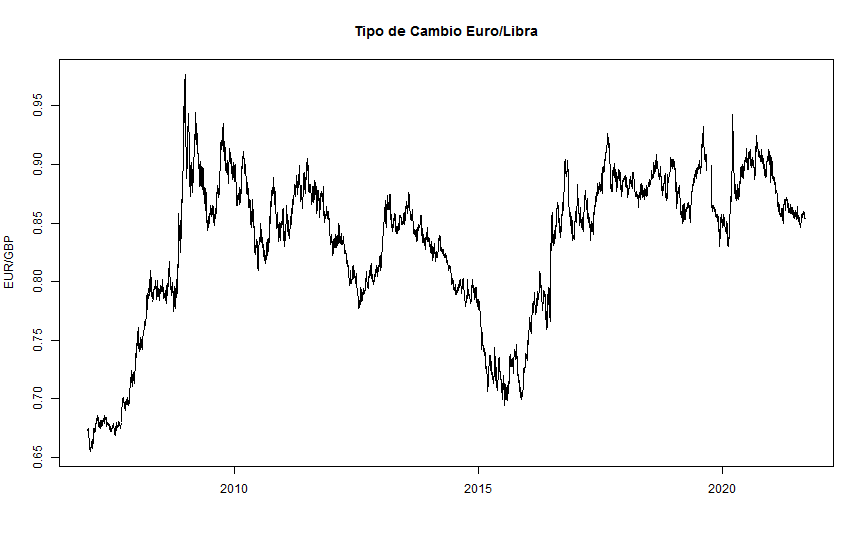
\includegraphics{Procesos_estocasticos_files/figure-beamer/er2-1} \end{center}

\end{frame}

\begin{frame}{Tipo de Cambio Nominal}

\begin{itemize}
\tightlist
\item
  El comportamiento del tipo de cambio es lejos de ser sistemático y
  predecible
\end{itemize}

\begin{center}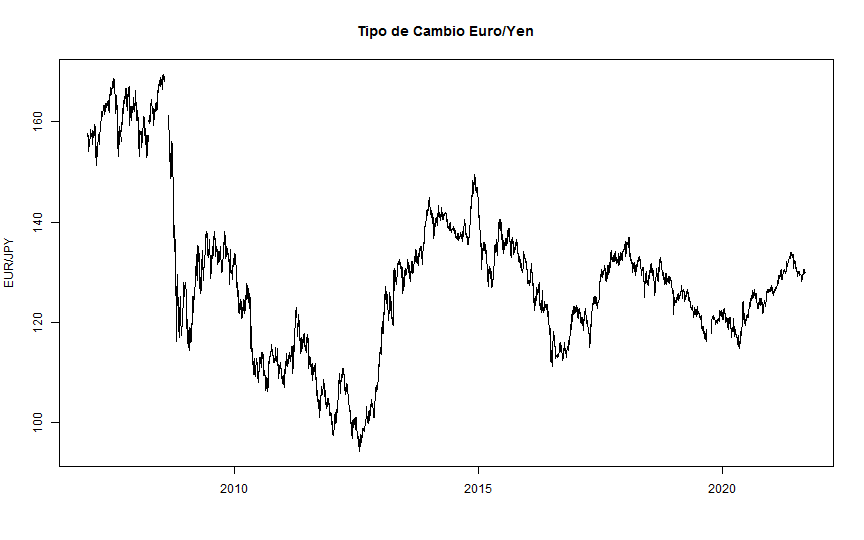
\includegraphics{Procesos_estocasticos_files/figure-beamer/er3-1} \end{center}

\end{frame}

\begin{frame}{Tipo de Cambio Nominal}

\begin{itemize}
\tightlist
\item
  Aunque sus variaciones presentan un comportamiento más predecible
\end{itemize}

\begin{center}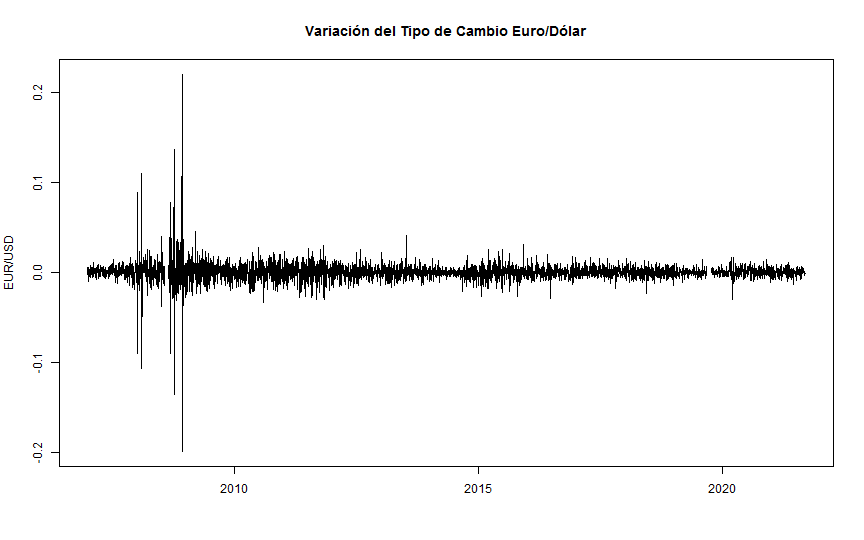
\includegraphics{Procesos_estocasticos_files/figure-beamer/er4-1} \end{center}

\end{frame}

\begin{frame}{Tipo de Cambio Nominal}

\begin{itemize}
\tightlist
\item
  Aunque sus variaciones presentan un comportamiento más predecible
\end{itemize}

\begin{center}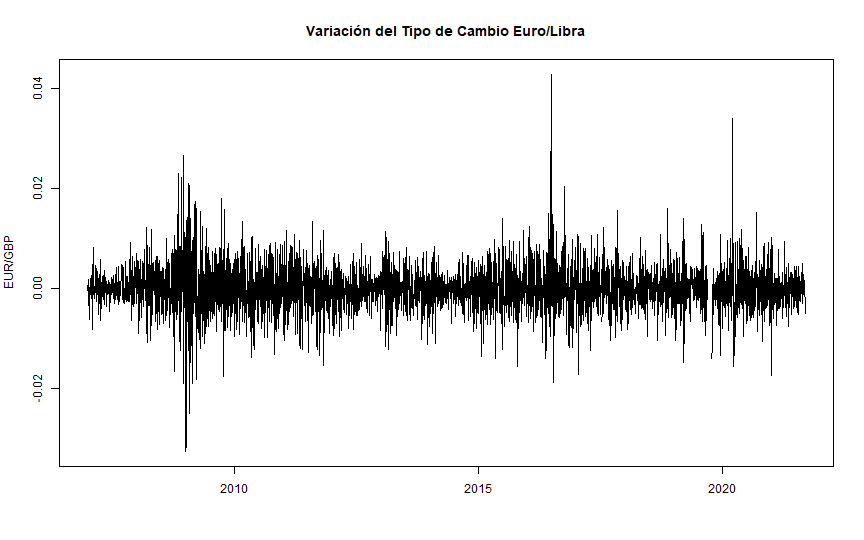
\includegraphics{Procesos_estocasticos_files/figure-beamer/er5-1} \end{center}

\end{frame}

\begin{frame}{Tipo de Cambio Nominal}

\begin{itemize}
\tightlist
\item
  Aunque sus variaciones presentan un comportamiento más predecible
\end{itemize}

\begin{center}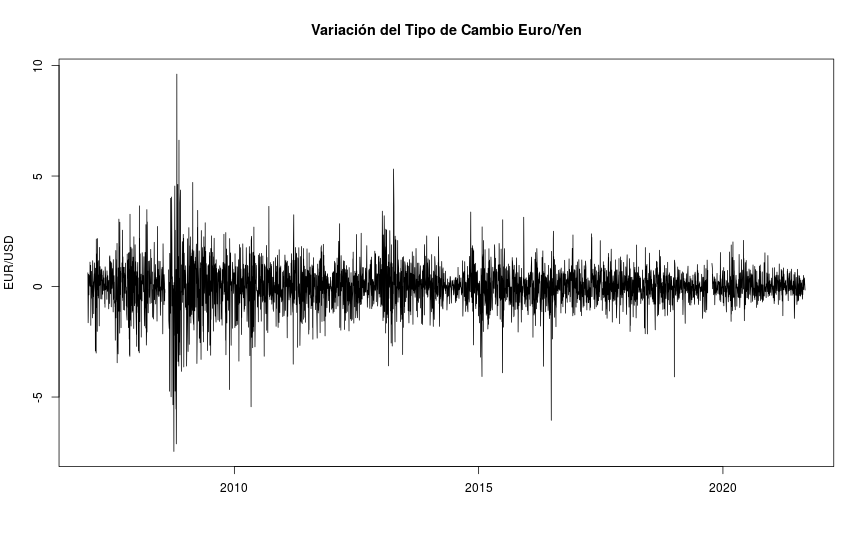
\includegraphics{Procesos_estocasticos_files/figure-beamer/er6-1} \end{center}

\end{frame}

\begin{frame}{Proceso estocástico y serie temporal}

\begin{itemize}
\item
  Una serie temporal es una colección de observaciones de una variable
  tomadas de forma secuencial y ordenada en el tiempo (instantes de
  tiempo equiespaciados). Las series pueden tener una periodicidad
  anual, semestral, trimestral, mensual, semanal, diaria etc., según los
  periodos de tiempo en los que están recogidos los datos que la
  componen.
\item
  Un proceso estocástico es una secuencia de variables aleatorias,
  ordenadas y equidistantes cronológicamente referidas a una
  característica observable en diferentes momentos.
\item
  Por ello, una serie temporal es una \textbf{realización particular de
  una muestra procedente de un proceso estocástico.}
\end{itemize}

\end{frame}

\begin{frame}{Proceso estocástico y serie temporal}

\begin{itemize}
\tightlist
\item
  Una serie temporal es una realización particular de un proceso
  estocástico
\end{itemize}

\begin{center}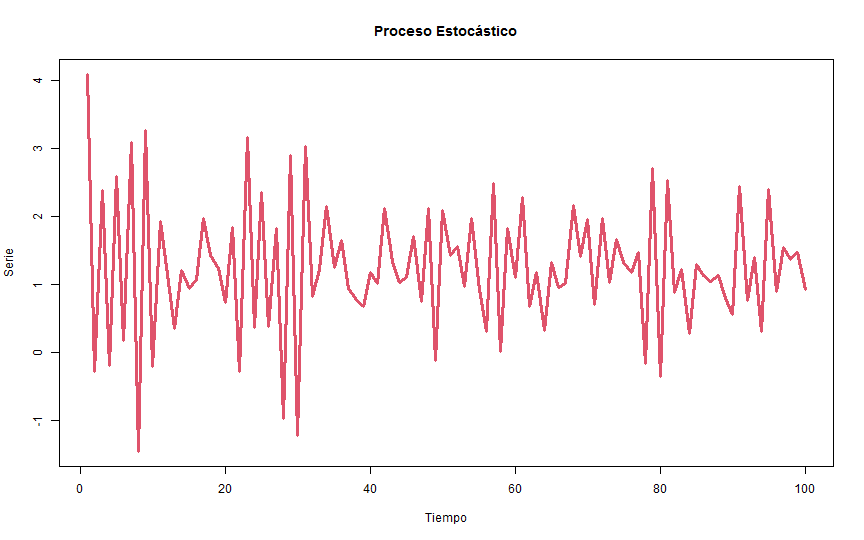
\includegraphics{Procesos_estocasticos_files/figure-beamer/proceso01-1} \end{center}

\end{frame}

\begin{frame}{Proceso estocástico y serie temporal}

\begin{itemize}
\tightlist
\item
  Una serie temporal es una realización particular de un proceso
  estocástico
\end{itemize}

\begin{center}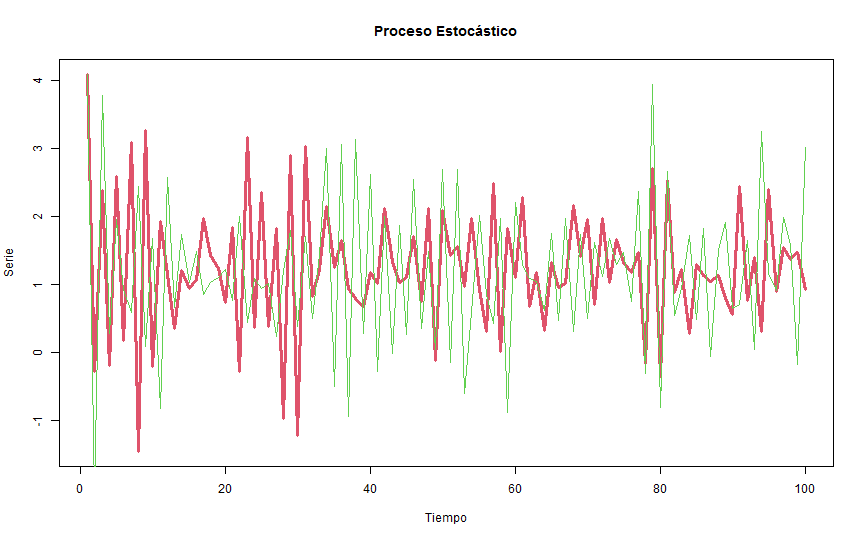
\includegraphics{Procesos_estocasticos_files/figure-beamer/proceso02-1} \end{center}

\end{frame}

\begin{frame}{Proceso estocástico y serie temporal}

\begin{itemize}
\tightlist
\item
  Una serie temporal es una realización particular de un proceso
  estocástico
\end{itemize}

\begin{center}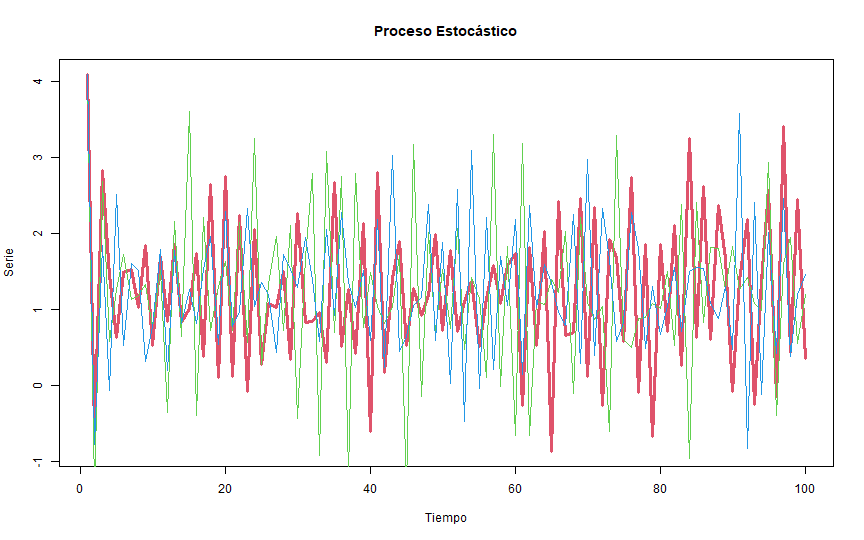
\includegraphics{Procesos_estocasticos_files/figure-beamer/proceso03-1} \end{center}

\end{frame}

\begin{frame}{Proceso estocástico y serie temporal}

\begin{itemize}
\tightlist
\item
  Una serie temporal es una realización particular de un proceso
  estocástico
\end{itemize}

\begin{center}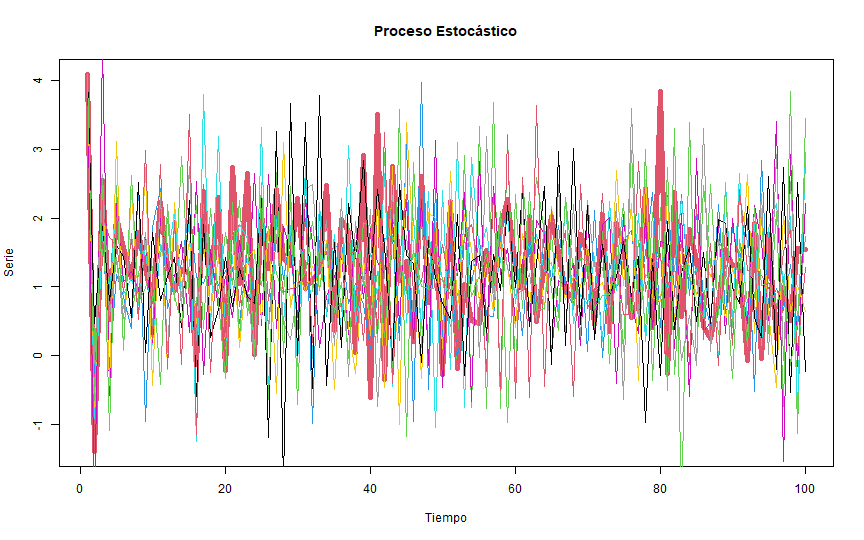
\includegraphics{Procesos_estocasticos_files/figure-beamer/proceso04-1} \end{center}

\end{frame}

\begin{frame}{Proceso estocástico y serie temporal}

\end{frame}

\begin{frame}{Proceso estocástico y serie temporal}

\begin{itemize}
\item
  Elaborar un \textbf{modelo estadístico} para una muestra procedente de
  un proceso estocástico \(Y_t\) a partir de una única realización
  particular (una serie temporal \(y_t\)).
\item
  Utilizar el modelo elaborado para \textbf{prever} los futuros valores
  de proceso \(Y_{(N+l)}\).
\item
  \textbf{Contrastar} alguna teoría sobre la característica o variable a
  la que se refiere la serie considerada.
\end{itemize}

\end{frame}

\begin{frame}{Proceso estocástico y serie temporal}

\begin{block}{¿Cómo lo vamos a hacer?}

\begin{itemize}
\item
  Para conseguir estos objetivos se va a seleccionar un modelo para la
  muestra dentro de una clase general de modelos denominados ARIMA, que
  implique cierta propiedades teóricas para el proceso estocástico
  \(Y_t\) del que procede la muestra y que resulten compatibles con las
  propiedades muestrales observadas en la serie temporal \(y_t\).
\item
  El problema para hacer esto es que solo tenemos una única realización
  particular del proceso estocástico. Para solucionar esto necesitamos
  que se cumpla la hipótesis de estacionariedad.
\end{itemize}

\end{block}

\end{frame}

\begin{frame}{Estacionariedad: Definición}

Si \(\{y_t\}\) es una serie temporal estacionaria, entonces para todo
\(s\), la distribución de \((y_t,\dots,y_{t+s})\) no depende de \(t\).

Una \textbf{serie estacionaria} es:

\begin{itemize}
\item
  aproximadamente horizontal
\item
  varianza constante
\item ~
  \subsection{no hay patrones predecibles a largo
  plazo}\label{no-hay-patrones-predecibles-a-largo-plazo}
\end{itemize}

\end{frame}

\begin{frame}{¿Estacionario?}

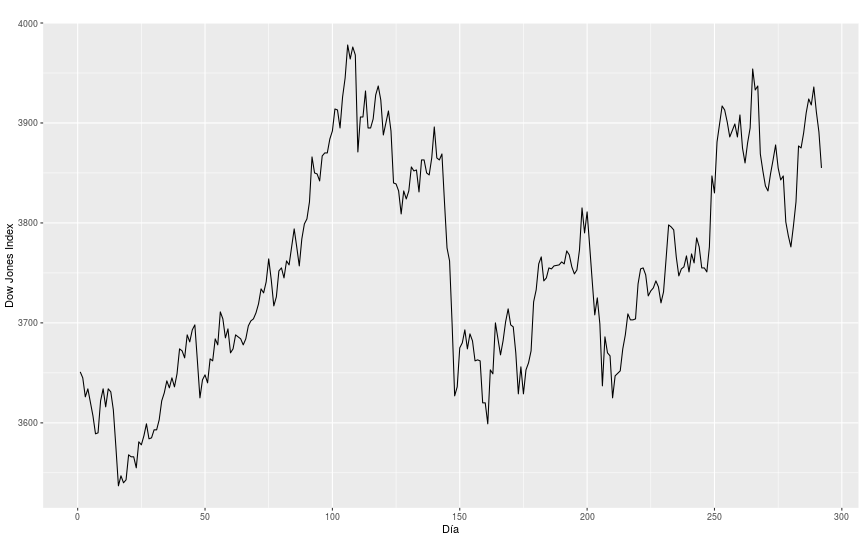
\includegraphics{Procesos_estocasticos_files/figure-beamer/unnamed-chunk-1-1.pdf}

\end{frame}

\begin{frame}{¿Estacionario?}

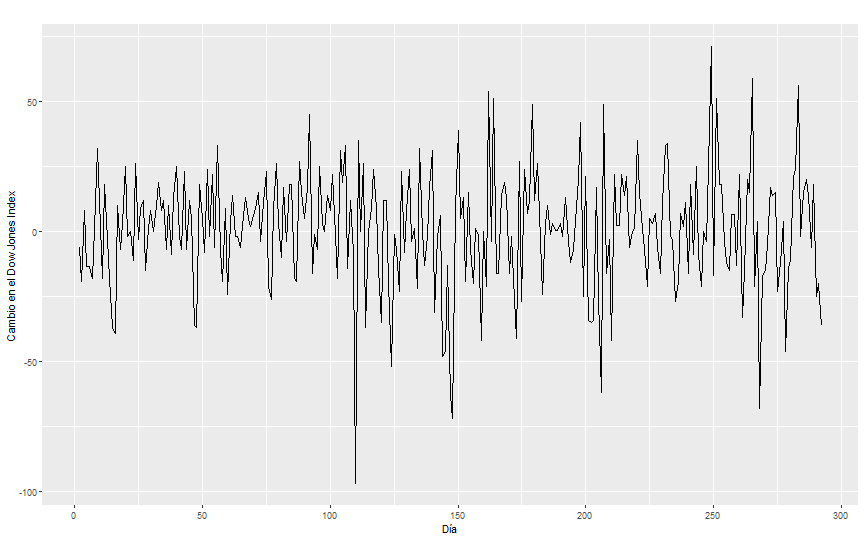
\includegraphics{Procesos_estocasticos_files/figure-beamer/unnamed-chunk-2-1.pdf}

\end{frame}

\begin{frame}{¿Estacionario?}

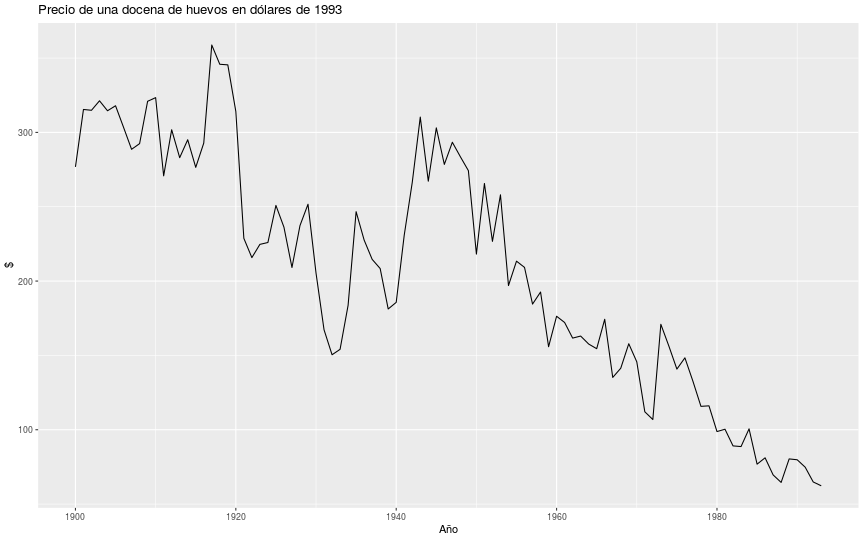
\includegraphics{Procesos_estocasticos_files/figure-beamer/unnamed-chunk-3-1.pdf}

\end{frame}

\begin{frame}{¿Estacionario?}

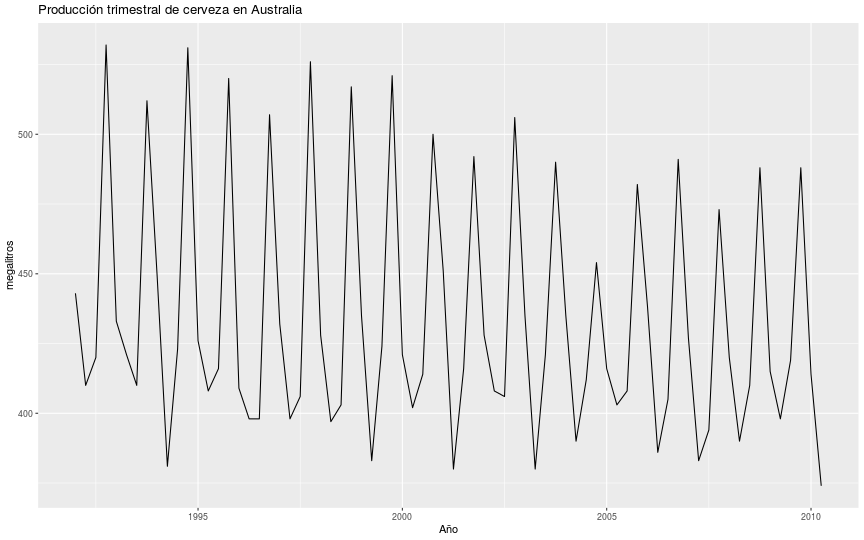
\includegraphics{Procesos_estocasticos_files/figure-beamer/unnamed-chunk-4-1.pdf}

\end{frame}

\begin{frame}{Propiedades de la hipótesis de estacionariedad}

\begin{itemize}
\item
  {\textbf{Estacionariedad}}: cierto estado de equilibrio estadístico
  que caracteriza la evolución temporal de un proceso estocástico que ha
  genera una serie temporal.
\item
  {\textbf{Media}}: valor constante en el tiempo que mide el nivel
  alrededor del cual evoluciona un proceso estocástico estacionario.
\item
  {\textbf{Varianza}}: valor constante en el tiempo que mide la
  dispersión o la variabilidad de la evolución temporal de un proceso
  estocástico estacionario alrededor de su media.
\item
  {\textbf{Autocorrelaciones}}: valores constantes en el tiempo que
  miden el grado de asociación lineal entre cada par de componentes de
  un proceso estocástico estacionario separados por diferentes
  intervalos temporales o retardos.
\end{itemize}

\end{frame}

\begin{frame}{Proceso ruido blanco}

\begin{itemize}
\item
  Ruido blanco \(x_t = w_t\)
\item
  Donde \(E(w_t)=0\;\;\; var(w_t)=\sigma^2 \;\;\; \forall t\)
\end{itemize}

\begin{center}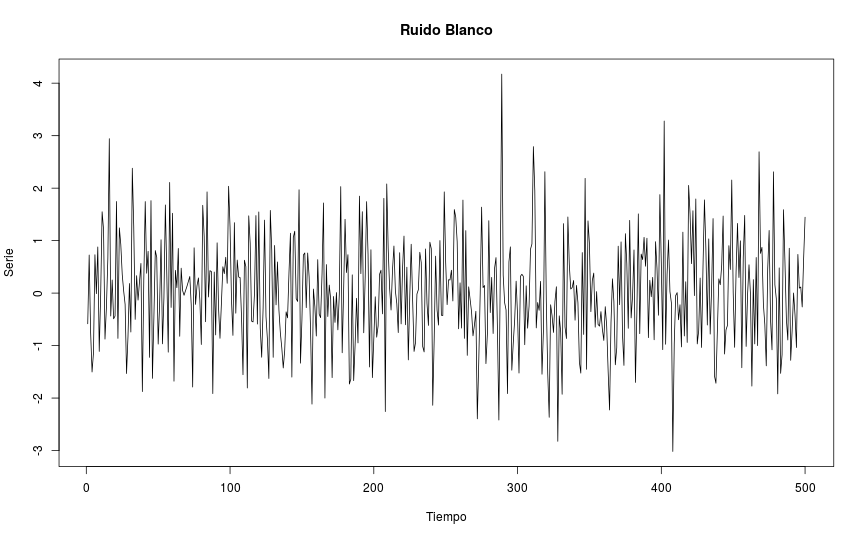
\includegraphics{Procesos_estocasticos_files/figure-beamer/ruido01-1} \end{center}

\end{frame}

\begin{frame}{Proceso ruido blanco}

\begin{itemize}
\tightlist
\item
  Lo vemos con menos datos para que se visalize mejor
\end{itemize}

\begin{center}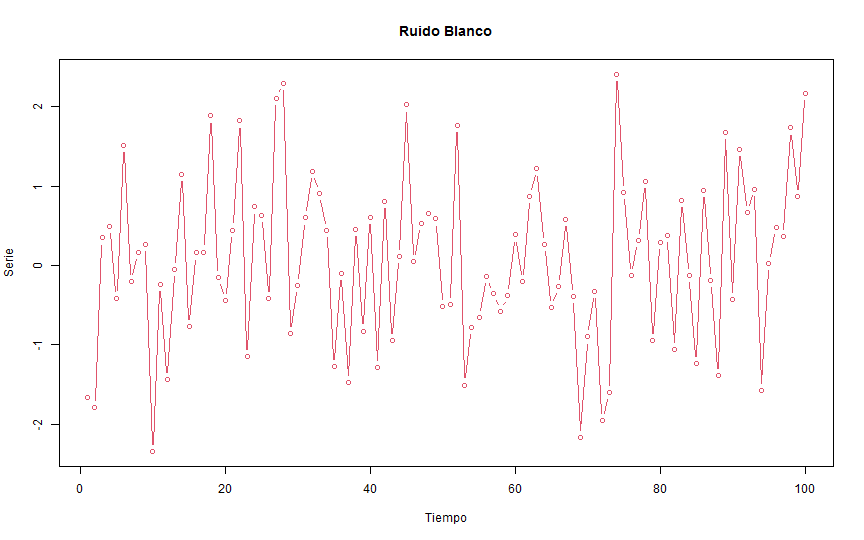
\includegraphics{Procesos_estocasticos_files/figure-beamer/ruido02-1} \end{center}

\end{frame}

\begin{frame}{Proceso ruido blanco con deriva (drift)}

\begin{itemize}
\tightlist
\item
  Ruido blanco con deriva \(x_t =\delta + w_t\)
\end{itemize}

\begin{center}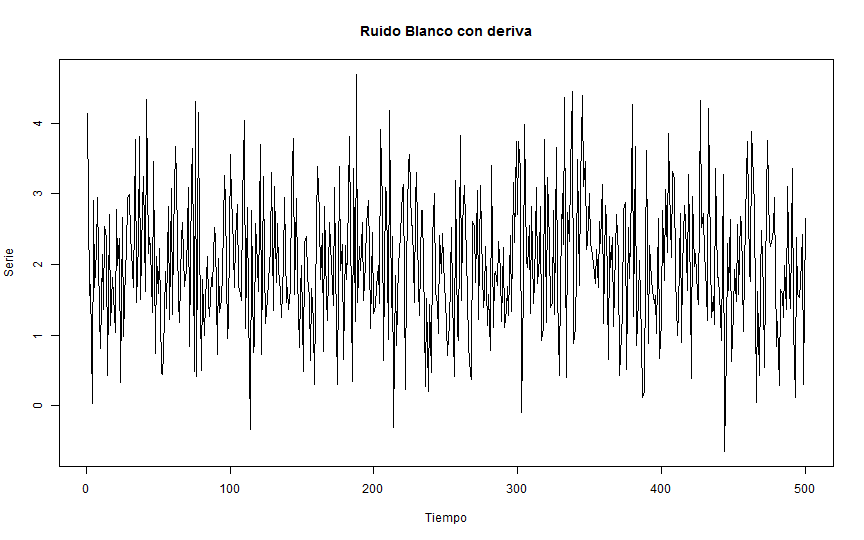
\includegraphics{Procesos_estocasticos_files/figure-beamer/ruido03-1} \end{center}

\end{frame}

\begin{frame}{Proceso media movil}

\begin{itemize}
\item
  Media móvil \(x_t = \theta w_t\)
\item
  En este caso particular el proceso es
  \(x_t =\frac{1}{3} (w_{t-1}+w_t+w_{t+1})\). Se puede interpretar como
  una media centrada en cada observación
\end{itemize}

\begin{center}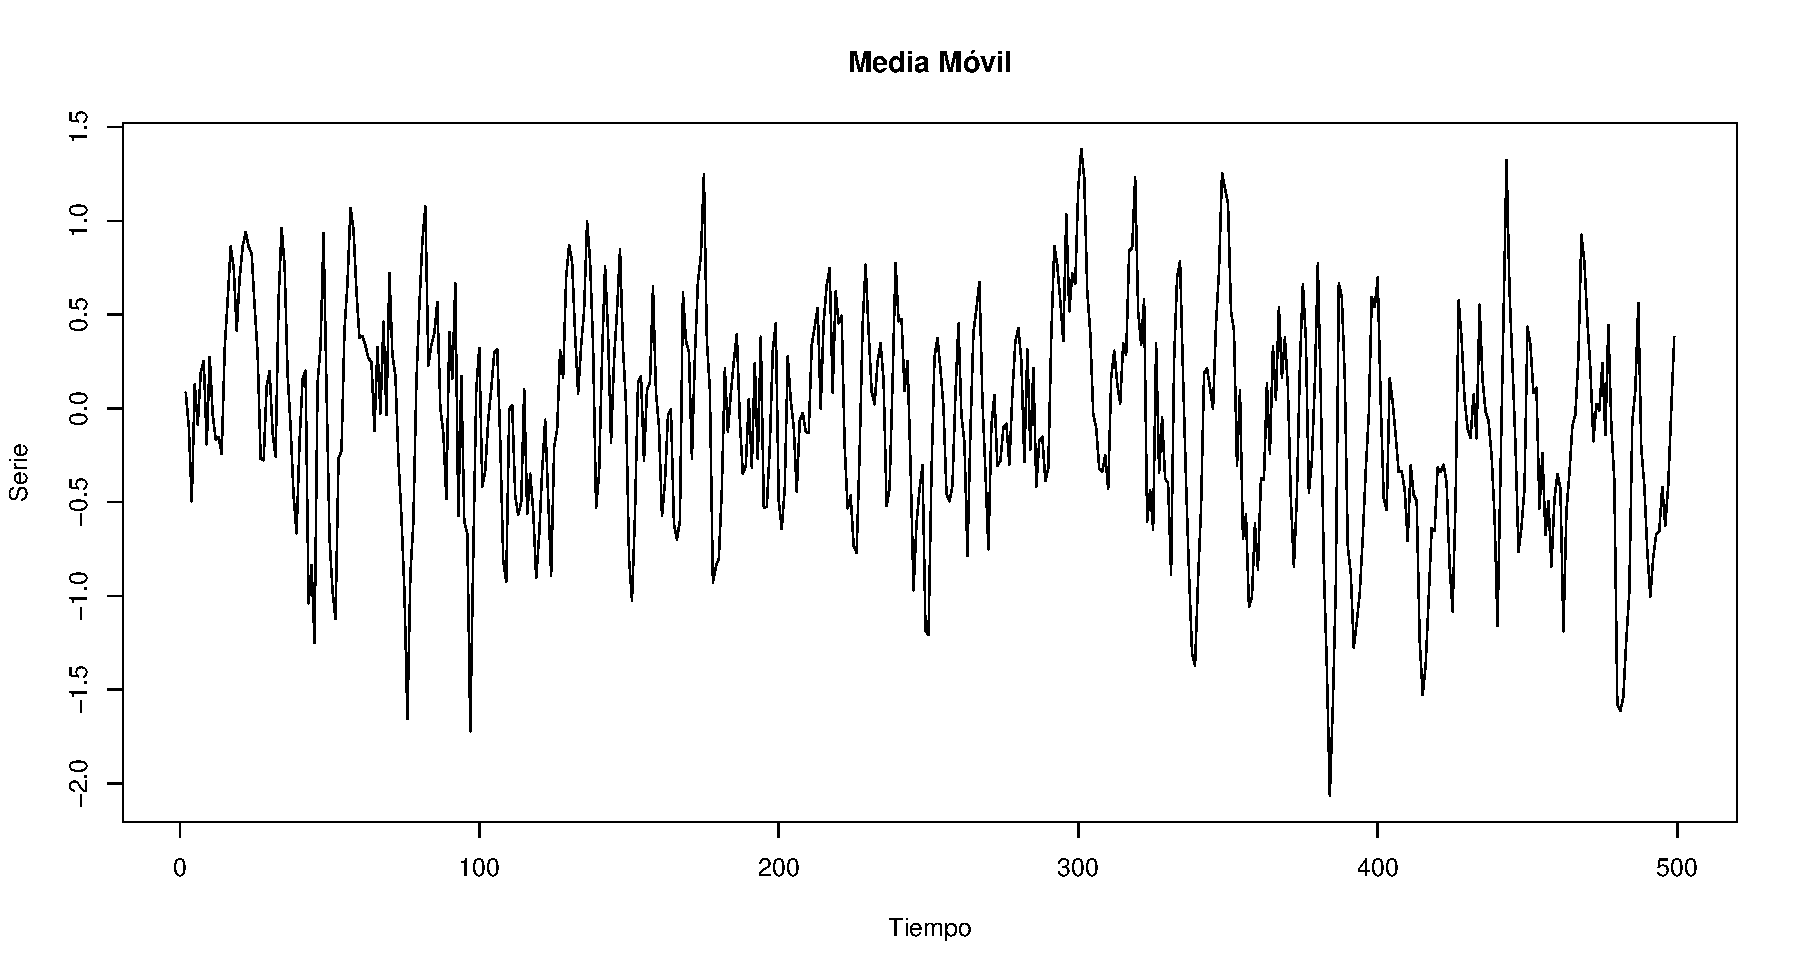
\includegraphics{Procesos_estocasticos_files/figure-beamer/ma01-1} \end{center}

\end{frame}

\begin{frame}{Ambos procesos}

\begin{center}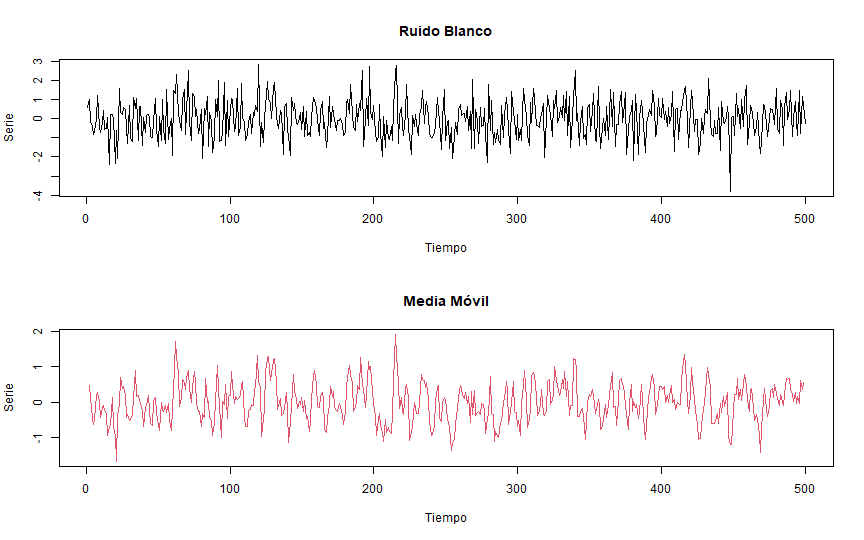
\includegraphics{Procesos_estocasticos_files/figure-beamer/ma02-1} \end{center}

\end{frame}

\begin{frame}{Procesos autoregresivos}

\begin{itemize}
\tightlist
\item
  Proceso autoregresivo de orden 2 \(x_t = x_{t-1} - 0.9x_{t-2} + w_t\)
\end{itemize}

\begin{center}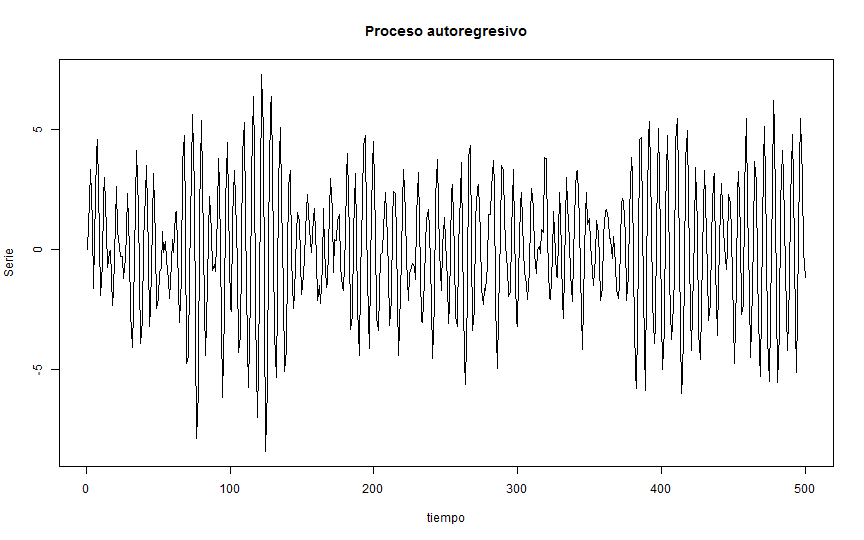
\includegraphics{Procesos_estocasticos_files/figure-beamer/ar01-1} \end{center}

\end{frame}

\begin{frame}{Random walk (Paseo aleatorio)}

\begin{itemize}
\item
  Paseo aleatorio \(x_t = x_{t-1} + w_t\)
\item
  Paseo aleatorio con deriva \(x_t = \delta+ x_{t-1} + w_t\)
\end{itemize}

\begin{center}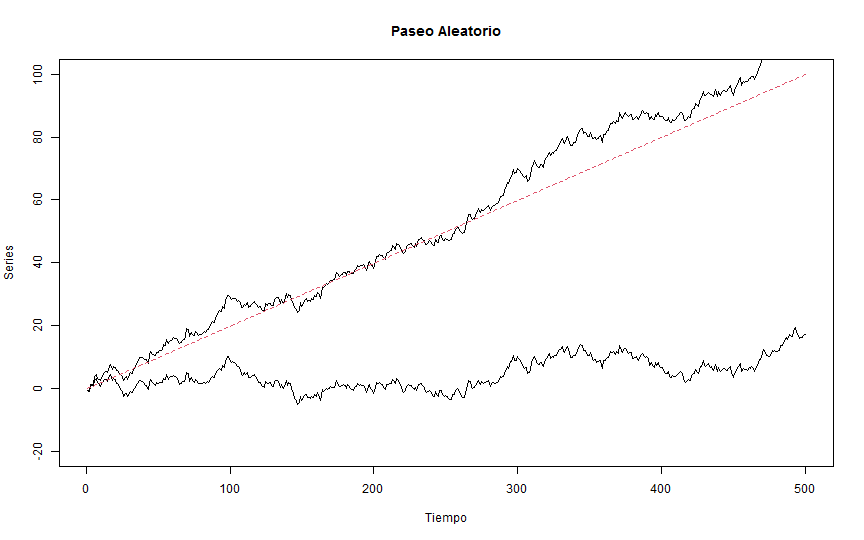
\includegraphics{Procesos_estocasticos_files/figure-beamer/rw01-1} \end{center}

\end{frame}

\end{document}
